\documentclass[11pt]{article}
\usepackage[top=0.9in, left=0.9in, bottom=0.9in, right=0.9in]{geometry}
\usepackage{graphicx}
\usepackage{booktabs}
\usepackage[numbers]{natbib}
\usepackage{hyperref}
\usepackage{amsmath}
\usepackage{placeins}

\title{\textbf{When Regulation Beats the Algorithm} \\ \large Where and When Yellow Taxi Drivers Should Queue for JFK Flat-Fare Trips}
\author{
Michael Vallen Suryajaya \\
{\small \url{https://github.com/michaelvallen14/nyc-taxi-jfk-flat-fare}} \\
\small (commit: 1ed92dc)
}
\date{\today}

\begin{document}
\maketitle

\section{Introduction}

Everyday, thousands of people face the same problem once they get off a plane at JFK
Airport. They can call a yellow taxi at a fixed rate or open a rideshare app (Uber,
Lyft, Juno, etc.), but they have to gamble on which one is actually cheaper.
Therefore, this project will find out under what demand conditions the regulated JFK
flat fare (RatecodeID 2) actually outperforms priced rideshare and how that should
change where yellow taxi drivers choose to position themselves.

RatecodeID 2 is a New York City Taxi and Limousine Commission (TLC) rule which fixes
the fare for any trip between the JFK airport and Manhattan at a same dollar amount,
regardless of traffic, time of day or distance. It is introduced to stop drivers' long
wait with unfamiliar travellers on a time-based meter \citep{tlc-fare-page}. This kind
of price regulation is well studied where regulated fares are known to create
frictions relative to a free-market price, but also to protect riders from the kind of
search-cost exploitation the flare fare targets \citep{frechette2019frictions}. The
other way for rideshare apps, they use surge pricing precisely because it lets
marketplace price move with real-time supply and demand, and drivers respond to it by
relocating toward higher demand areas \citep{garg2022driversurge}. Standard metered
fares and rideshare fares carry no price-fixing protection, so they should respond to
demand. This project will test whether that is actually true in the data, and if so,
when. Hence the target audience for this project, the yellow taxi drivers and fleet
dispatchers deciding whether, and when, to queue at JFK rather than work elsewhere in
the city.

The primary dataset is NYC TLC Yellow Taxi trip records for January until June 2025
(24,083,384 raw trips) \citep{tlc-trip-data}. The secondary dataset is the comparison
group of NYC TLC High Volume For-Hire Vehicle (HVFHV) trip records for the same window
(120,995,191 raw trips) representing dynamically priced rideshare. The six-month
window satisfies the Project's PySpark minimum. 2025 was chosen because Manhattan's
congestion pricing began on January 5th and ran through the entire study period. This
makes January-June 2025 a single uninterrupted fare regime with a live
regulated-pricing feature, the
\texttt{cbd\_congestion\_fee}, and one that is itself the subject of ongoing
transportation-economics research into whether it changes ride-hailing and taxi
behaviour in the city \citep{li2024congestionfees}. Lastly, the external dataset is
the US Bureau of Transportation Statistics' (BTS) Airline On-Time Performance data for
January--June 2025 \citep{bts-ontime}, used to measure actual JFK flight arrival
volume and delay as a proxy for passenger demand.

\textbf{Feature of Interest:}
\begin{itemize}
  \item \texttt{RatecodeID} (1-6) : the fare regime for a yellow taxi trip
  \item \texttt{fare\_amount} and \texttt{base\_passenger\_fare} : prices paid for a trip
  \item \texttt{PULocationID} : locate pickups location
  \item \texttt{DOLocationID} : locate drop-offs location
\end{itemize}

Uber,Lyft and other rideapps are grouped together instead of being split by company
because a driver waiting at the airport doesn't know which specific app is busy and
also each driver can open multiple apps at once. Flight arrival times are also
shifted forward by one hour to estimate when passengers actually reach the taxi line
and since people need time to leave the plane, collect bags and walk outside. This
one-hour shift is only an assumption, not an exact measurement. Two limitations of
the BTS data are worth noting: it counts flights, not passengers, and only includes
domestic flights, so flight counts are used as a relative demand proxy rather than
an exact passenger count \citep{bts-ontime}.

The project begins by verifying and cleaning both TLC taxi datasets according to
their official rulebooks, eliminating invalid or unusable entries from the yellow
taxi and HVFHV data (Section 2). It then combines the taxi data with flight arrival
data from the US Bureau of Transportation Statistics, matched by hour to see how taxi
and rideshare prices change depending on how many flights are landing at JFK (Section
3). Then a geographic breakdown of trip destinations checks whether the taxi flat
fare's low price variation is a real effect of NYC's flat-fare rule or just because
those trips happen to go to similar places ( Section 3 ). Two models are then used,
linear regression and a random forest, then predict hourly average rideshare fare from
flight arrival volume, arrival delay, hour of day and day of week which will answer
when the \$70 flat fare beats rideshare pricing (Section 4). All of this will converge
with recommendations for yellow taxi drivers and fleet dispatchers deciding when to
queue at JFK (Section 5).

\section{Preprocessing}

The dataset collected is real-time sensors and it doesn't guarantee its accuracy
\citep{tlc-trip-data}, which preprocessing is required to address potential invalid
analysis or inconsistencies. The steps below outline the preprocessing procedures
applied to remove invalid data:

\subsection{Yellow Taxi Trip Records}

\begin{itemize}
  \item \textbf{Invalid location:} Zone codes with number 264 and 265 for pickup or
    drop-off is removed since it is not real NYC zones (Borough = ``Unknown'').
  \item \textbf{Missing fare type:} Ratecode with ID of 99 means ``Null/unknown''
    \citep{tlc-yellow-dict} and a trip with no clear fare type can't be used for this
    project.
  \item \textbf{Negative fare amounts and fee-related fields:} Any trip record
    containing negative values in fare amounts or associated fee fields is considered
    invalid and removed.
  \item \textbf{Negative trip distance:} it's not possible to have a negative distance
    for a trip. This could be cancelled trips or clock errors.
\end{itemize}

The window kept is 1 January to 30 June 2025 inclusive. The first four of these 181
days predate Manhattan's congestion pricing scheme, which began 5 January 2025; this
is a negligible share of the window and is stated here rather than silently dropped.

\begin{table}[h]
\centering
\caption{Yellow taxi shape at each filtering step}
\label{tab:yellow-shape}
\small
\begin{tabular}{lrr}
\toprule
Step & Rows remaining & Rows dropped \\
\midrule
Raw, Jan--Jun 2025 & 24,083,384 & -- \\
Drop unknown zone codes (264/265) & 23,904,717 & 178,667 \\
Drop null/unknown RatecodeID (99, null) & 18,233,691 & 5,671,026 \\
Drop non-positive fare\_amount & 17,825,652 & 408,039 \\
Drop non-positive trip\_distance & 17,635,957 & 189,695 \\
Drop non-positive trip duration & 17,446,797 & 189,160 \\
Restrict to Jan--Jun 2025 window & 17,446,773 & 24 \\
\bottomrule
\end{tabular}
\end{table}

\FloatBarrier

\subsection{High Volume For-Hire Vehicle (HVFHV) Trip Records}

The HVFHV dataset, representing dynamically priced rideshare, is preprocessed following
identical logic against the HVFHV data dictionary \citep{tlc-hvfhs-dict}:

\begin{itemize}
  \item \textbf{Invalid location:} Zone codes with number 264 and 265 for pickup or
    drop-off, for the same reason as yellow taxi.
  \item \textbf{Negative base fare:} the base fare before tolls, tips, taxes and fees is
    considered invalid and removed if there's a non-positive
    \texttt{base\_passenger\_fare}, the same as the yellow taxi \texttt{fare\_amount}
    filter.
  \item \textbf{Negative trip distance and duration:} non-positive \texttt{trip\_miles}
    and \texttt{trip\_time} are removed, just like yellow taxi.
\end{itemize}

\begin{table}[h]
\centering
\caption{HVFHV shape at each filtering step}
\label{tab:hvfhv-shape}
\small
\begin{tabular}{lrr}
\toprule
Step & Rows remaining & Rows dropped \\
\midrule
Raw, Jan--Jun 2025 & 120,995,191 & -- \\
Drop unknown zone codes (264/265) & 115,684,444 & 5,310,747 \\
Drop non-positive base\_passenger\_fare & 115,580,227 & 104,217 \\
Drop non-positive trip\_miles & 115,565,413 & 14,814 \\
Drop non-positive trip\_time & 115,565,413 & 0 \\
Restrict to Jan--Jun 2025 window & 115,565,413 & 0 \\
\bottomrule
\end{tabular}
\end{table}

\FloatBarrier

\subsection{BTS Airline On-Time Performance Data}

Since the BTS dataset covers all US domestic flights rather than only those relevant to
this study, two filtering steps are applied:

\begin{itemize}
  \item \textbf{Non-JFK arrivals:} flights arriving at airports other than JFK
    (\texttt{Dest != "JFK"}) are removed, since this project is only concerned with the
    airport where the flat fare applies.
  \item \textbf{Cancelled or diverted flights:} these never land, so they generate no
    curb pickups and have no meaningful arrival delay, and are therefore removed
    \citep{bts-ontime}.
\end{itemize}

This large reduction reflects narrowing from all US domestic flights nationwide down to
only those landing at JFK, not a data-quality issue (Table~\ref{tab:bts-shape}).

\begin{table}[h]
\centering
\caption{BTS shape at each filtering step}
\label{tab:bts-shape}
\small
\begin{tabular}{lrr}
\toprule
Step & Rows remaining & Rows dropped \\
\midrule
Raw, all US domestic flights, Jan--Jun 2025 & 3,446,676 & -- \\
Filter to flights arriving at JFK & 51,395 & 3,395,281 \\
Drop cancelled/diverted flights & 50,586 & 809 \\
\bottomrule
\end{tabular}
\end{table}

\FloatBarrier

\section{Analysis and Geospatial Visualisation}

\subsection{Fare Variance by Pricing Mechanism}

\begin{table}[h]
\centering
\caption{Full-distribution fare statistics at JFK, Jan--Jun 2025}
\label{tab:fare-stats}
\small
\begin{tabular}{lrrrr}
\toprule
Pricing mechanism & $n$ & Mean (\$) & Std. dev. (\$) & CV \\
\midrule
Yellow taxi -- flat fare & 457,903 & 70.00 & 0.10 & 0.0015 \\
Yellow taxi -- standard metered & 363,899 & 49.56 & 23.69 & 0.478 \\
Rideshare (HVFHV) & 1,688,161 & 61.50 & 32.37 & 0.526 \\
\bottomrule
\end{tabular}
\end{table}

Looking at Table~\ref{tab:fare-stats}, it shows the full-distribution fare statistics
for the 3 pricing mechanism at JFK. In this analysis we will use coefficient of
variation which is the standard deviation divided by mean to scale measure of price
variability. The flat fare's coefficient of variation is the lowest of all three at 0.0015,
around 300 times smaller than the other pricing mechanisms. There are small
number of flat fare trips that sit above \$70 (max \$86.69), there are not assumed,
these are confirmed and could be due to tolls and surcharges stacked on top of the base
amount for 0.017\% of trips, the base fare itself is untouched.

\begin{figure}[h]
\centering
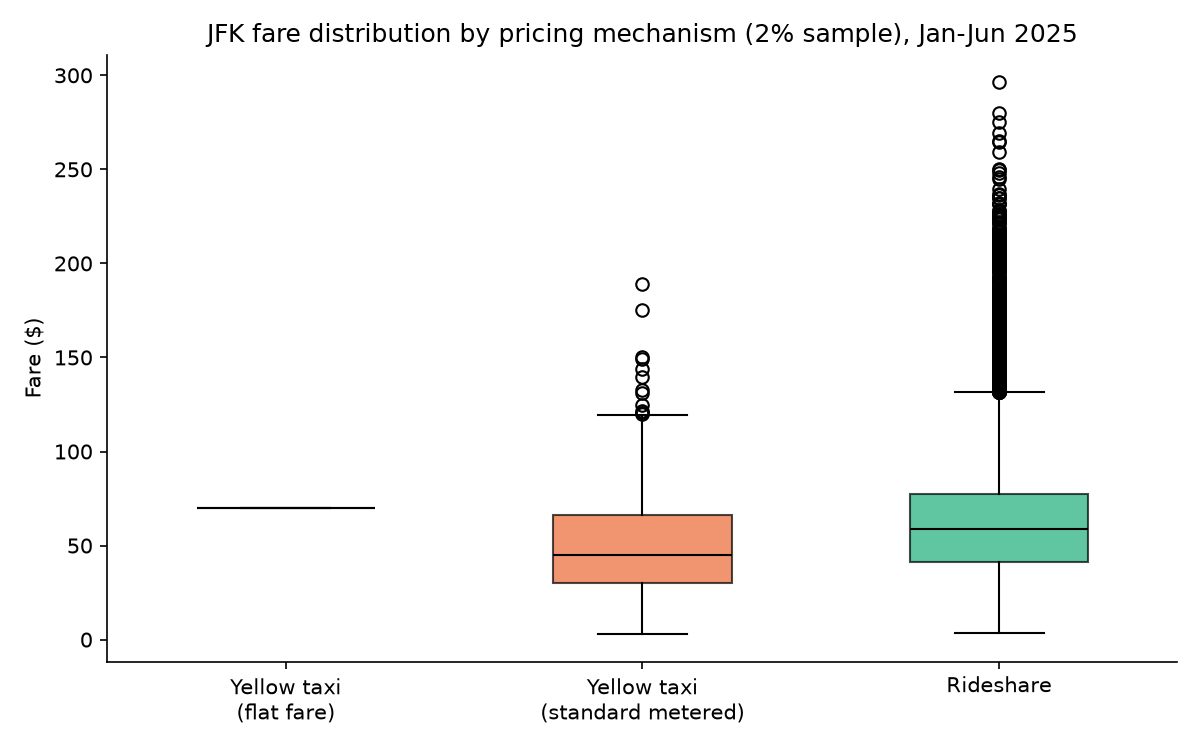
\includegraphics[width=0.5\textwidth]{plots/jfk_fare_variance_boxplot.png}
\caption{JFK fare distribution by pricing mechanism, 2\% sample for visualisation
(full-distribution statistics in Table~\ref{tab:fare-stats}).}
\label{fig:box}
\end{figure}

From Figure~\ref{fig:box} we can see that flat fare is near-invisible line at \$70,
therefore this outlier check itself, there is nothing to chase in the flat-fare tail
because a fixed price structurally cannot produce the long right tail other pricing
mechanism do. Both of the show a heavy tail of trips, especially for rideshare where
the tail is well above \$150. That tail is a genuine candidate for further work eg.
whether it is driven by a specific time, destination or other occasional surge
multipliers. Pursuing this is out of scope since the project's focus is the hour-by-hour
pattern.

\FloatBarrier

\subsection{Demand-Responsiveness}

\begin{figure}[h]
\centering
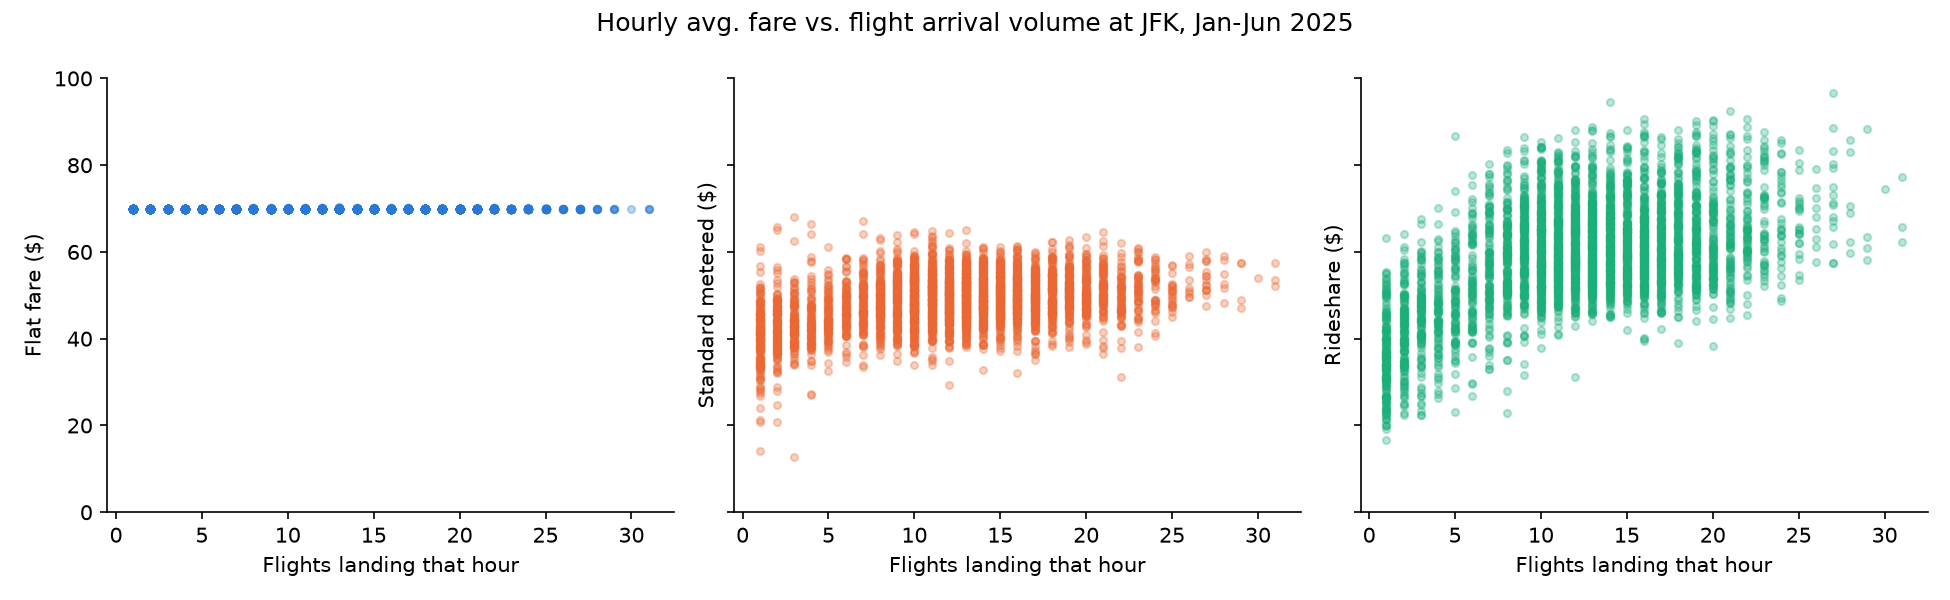
\includegraphics[width=0.85\textwidth]{plots/jfk_demand_vs_price.png}
\caption{Hourly average fare vs flight arrival volume at JFK by pricing mechanism}
\label{fig:demand}
\end{figure}

From Figure~\ref{fig:demand}, it is shown that flat fare also has the lowest and almost
no relationship with flight volume (r=0.023) compared to rideshare (r=0.536) and
standard metered (r=0.385). This data shows that rideshare is the only mechanism that
has relationship to real-time demand, perhaps because surge algorithms react directly
and differently, depends on the time of the day, to pickup request at the terminal
while the flat fare is fixed regardless of how many flight just landed. This shows as
an interaction, not a shared trend. The relationship between flight volume and price
depends on which pricing mechanism is being used, that's the reason rideshare's slope is
steep, an interaction effect that a single correlation pooled across all trip types
would have hidden entirely. It is convincing enough to pursue further, if flight volume
predicts rideshare price this cleanly in aggregate, it should also be usable to predict
price directly by hour.

\subsection{Geospatial Destination Analysis}

RatecodeID at JFK is mostly destination-determined rather than a free pricing choice
based on the Geospatial analysis. From Figure~\ref{fig:borough}, it is visible that
98.9\% of flat-fare trips go to Manhattan, while standard metered trips go mostly to
Queens (52\%) and Brooklyn (41.1\%).

\begin{figure}[h]
\centering
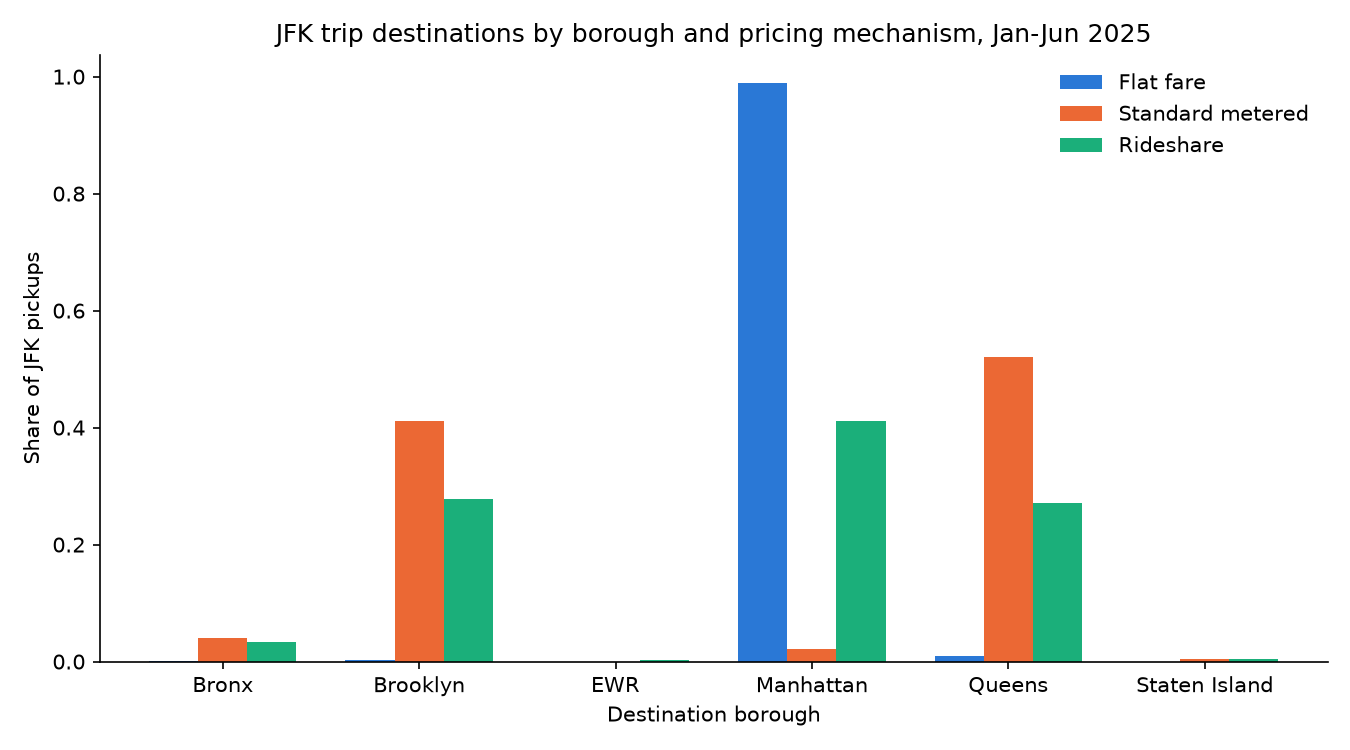
\includegraphics[width=0.58\textwidth]{plots/jfk_destination_borough.png}
\caption{JFK trip destinations by borough and pricing mechanism.}
\label{fig:borough}
\end{figure}

This is mostly because passengers going to Manhattan see the flat fare as a better
deal than gambling on price with a standard meter, which can rack up extra costs from
tolls and time spent in traffic. TLC's flat-fare rule is specifically
scoped to JFK-Manhattan trips \citep{tlc-fare-page}, while Queens or Brooklyn trip
cannot be flat-fare,regardless the demand.. From JFK to manhattan takes around 30-45
minutes on average, but if theres traffic or something unexpected involved, it could be
more than that and hence the price, something that human has no control over with. The
near-zero result for EWR and Staten Island in the Figure need no further investigation
since they are exactly what JFK's geography predicts.

\begin{figure}[h]
\centering
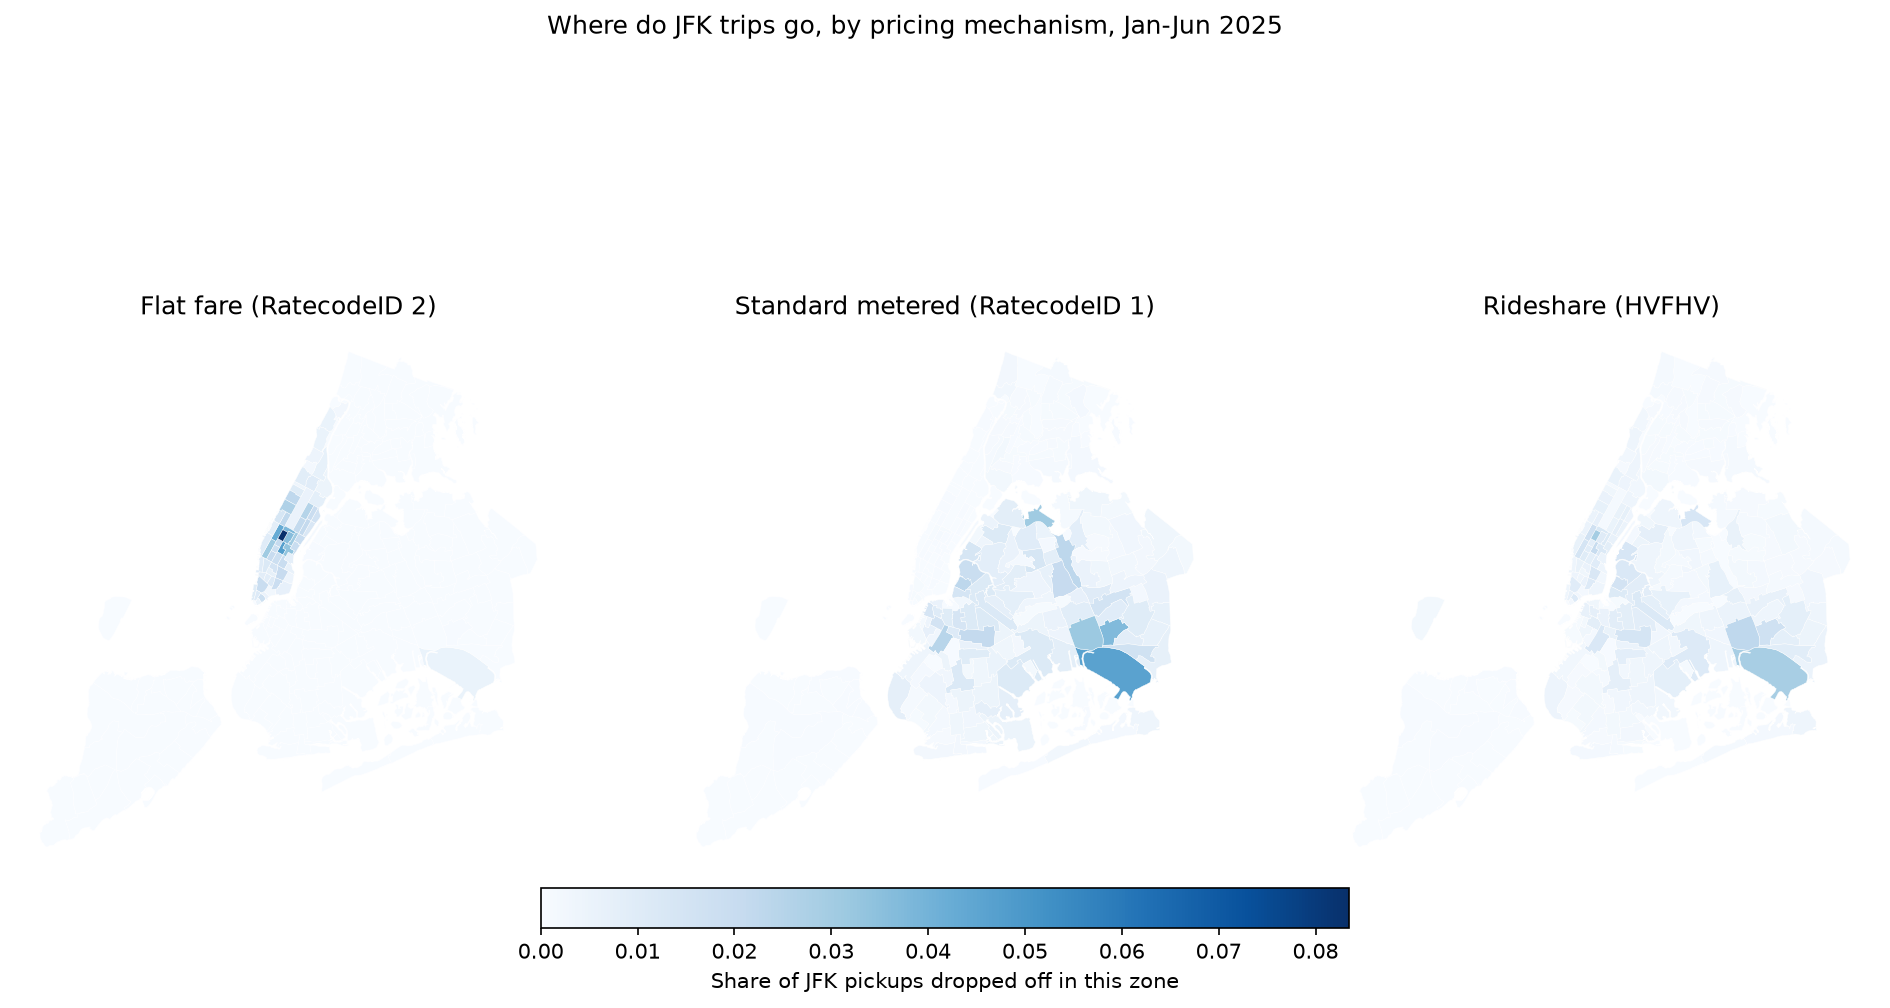
\includegraphics[width=0.85\textwidth]{plots/jfk_destination_choropleth.png}
\caption{Share of JFK pickups dropped off in each zone, by pricing mechanism (shared
colour scale).}
\label{fig:choropleth}
\end{figure}

From Figure 4, we can see flat-fare drop-offs concentrate heavily in just three central
Manhattan zones which include Times square (8.3\%), Midtown South (4.7\%), Clinton East
(4.3\%), touching only 223 distinct zones citywide compared for the other two
mechanisms. This happens perhaps because it skews toward Manhattan hotel and business
travellers rather than locals going to their home-address trips which could be mostly
with rideshare or standard metered. This concentration is itself an interesting avenue
for future research linking it to hotel or office density by zone rather than leaving
it as a blurry inference, doing so also need more external dataset outside this
project's scope.

\FloatBarrier

\section{Modelling}

For modelling, we'll use two models to predict \texttt{avg\_hvfhv\_fare} from four
predictors: \texttt{n\_flights}, \texttt{avg\_arr\_delay\_min}, \texttt{hour\_of\_day},
and \texttt{day\_of\_week}. Both models
will used data from January - April 2025 for training and May-June 2025 for testing.
Using temporal split rather than $k$-fold cross-validation on a random shuffle is more
practical since we're predicting future hours from past ones. Unlike random shuffle, it
tends to let the model see data from the same day it is being tested on which
overstating real-world accuracy. Hence model accuracy will be assessed using
MAE,RMSE and $R^2$. In this project, we will compare linear regression against a
random forest rather than other candidates and since the target is a continuous fare,
count model such as Poisson regression is not the right fit and it would risks
overfitting. Linear regression and random forest on the other hand, sit at opposite
ends of interpretability flexibility trade-off that matters most. The linear model's
coefficients capable to show directly which conditions move price, while random forest
will test whether a more flexible model captures more signal than the simpler one
misses.

\subsection{Models}

Firstly, we'll start with a simple linear regression model for predicting hourly
rideshare fare \citep{seghouane2023linearregression}:

\begin{equation}
\hat{y}_i = \beta_0 + \beta_1 x_{i1} + \beta_2 x_{i2} + \cdots + \beta_p x_{ip} +
\varepsilon_i,
\label{eq:linear}
\end{equation}

where $\hat{y}_i$ denotes the predicted average rideshare fare in hour $i$, $\beta_0$
is the intercept and $\beta_j$ are the coefficients for predictors $x_{ij}$ such as
flight volume, arrival delay, hour of day, or day of week and $\varepsilon_i$ is the
error term.

Linear regression typically relies on the assumption of additive relationship between
all the predictors and the outcome \citep{seghouane2023linearregression}. While in
reality, rideshare pricing could be
influenced by non-linear interactions such as delay or flight volume which the model
may not fully capture how these conditions combine to price. Therefore we deploy a
random forest, an ensemble of $T$ regression trees which to predict fare as their
average:

\begin{equation}
\hat{y}_i = \frac{1}{T} \sum_{t=1}^{T} f_t(x_i),
\label{eq:forest}
\end{equation}

where each $f_t$ is a regression tree fitted on a bootstrap sample of the training
data and $x_i$ is the same predictor vector used in Equation~\ref{eq:linear}.
Averaging many trees reduces the variance of any single tree's prediction, and each
tree can split on non-linear thresholds and interactions. The forest is fitted with
200 trees and a max depth of 8. To reduce the risk of overfitting, the depth is
capped deliberately since the training set is only 2,721 hourly observations.

\subsection{Results and Discussion}

Table~\ref{tab:models} shows the model comparison between Linear regression and
Random forest. They both have a similar result, but linear regression slightly
outperforms the random forest on the test period. Separate from hour-of-day and
flight-volume effects, It suggest the relationship between demand conditions and
rideshare price is mostly additive rather than requiring complex interactions a tree
ensemble. With the correlation already found in Section 3, random forest shows flight
volume is the dominant feature.

\begin{table}[h]
\centering
\caption{Model comparison, May--June 2025 test period}
\label{tab:models}
\small
\begin{tabular}{lrrr}
\toprule
Model & MAE (\$) & RMSE (\$) & $R^2$ \\
\midrule
Linear regression & 6.61 & 8.27 & 0.578 \\
Random forest & 7.01 & 8.76 & 0.527 \\
\bottomrule
\end{tabular}
\end{table}

From plotting, both models track the daily rise-and-fall rhythm closely which is
predicted against actual hourly fares over the test period. However, there's a minor
issue for this project, both models under-predict the highest daily peaks since it
makes the \$70 estimate below if anything conservative rather than inflated. This
also shows whether a driver does not need a complex model about JFK pricing since
time of day and flight volume already explain most of what is predictable about
rideshare price at the airport. Figure~\ref{fig:advantage} directly shows the
audience actually needs, not a model accuracy score, but a queuing schedule. It
shows that across the full six-month observed period, rideshare becomes more
expensive than the \$70 flat fare most reliably between 2pm and 6pm, with the peak
falling at 4-5pm (65-67\% of hours). While overnight (11pm-6am), rideshare almost never exceeds the
flat fare (under 5\% of hours, often exactly 0\%). Therefore, a taxi driver can act
on directly is that 4-5pm is worth prioritising and 2am is not.

\begin{figure}[h]
\centering
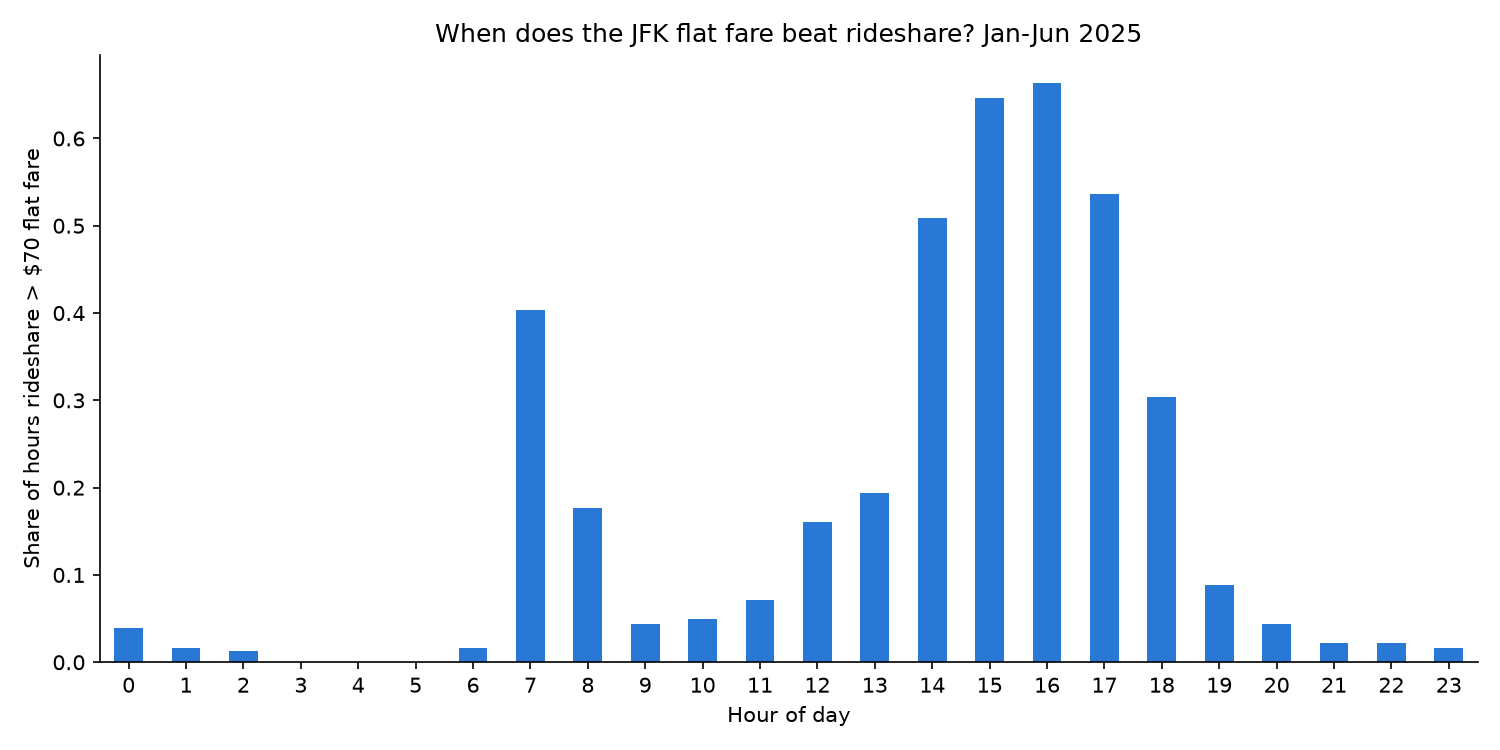
\includegraphics[width=0.62\textwidth]{plots/jfk_flat_fare_advantage_by_hour.png}
\caption{Share of hours rideshare exceeds the \$70 flat fare, by hour of day,
Jan--Jun 2025.}
\label{fig:advantage}
\end{figure}

\FloatBarrier

\section{Recommendations}

\textbf{Queue at JFK during the busy window (2-6pm), not "during the day"
generically.} From our modelling it is shown that the flat fares advantage peaks
sharply at 4-5pm which is around 65-67\% of the total hours and falls off quickly
outside this time window, a specific window to prioritise and not a restatement of
"avoid overnight shifts". Based on Section 3's r=0.536 correlation with flight
volume, this creates the window precisely, rideshare is demand-responsive, while the
flat fare is not. The model's hour-by-hour breakdown is that same
demand-responsiveness made precise enough to act on.

\textbf{Work in Manhattan instead of going back to the airport.} From previous
analysis, it is shown that the typical flat-fare drop-off location from JFK lands in
most part of Central Manhattan zones which includes Times Square (8.3\%), Midtown
South (4.7\%) and Clinton East (4.3\%). Meanwhile, drop-off location for standard
metered would normally make its way to Queens or Brooklyn with 93.1\% combined and
since next fare is less certain, going back to Manhattan could be worth it. This is
doubly true from Recommendation 1 where a driver finishing a flat-fare run then is
dropped in Manhattan at exactly the hours the model shows rideshare is most likely to
be overpriced, making it the worst possible time to head back to a queue instead of
picking up locally. This matches prior modelling of NYC taxi drivers' own
airport-return decisions, where spatial proximity and prior drop-off location were
the strongest predictors of that choice \citep{yazici2016jfk}. Another onward
opportunity claim also can be made since the yellow taxi nor HVFHV data carries a
driver or vehicle identifier.

\section{Conclusion}

In conclusion, this project found an answer with strong evidence to determine when
the JFK flat fare actually outperforms standard-metered and rideshare prices. Based
on the analysis I've put up, the flat fare's advantage is not constant, its only
concentrated in a specific mid-afternoon-to-evening window, to be exact at 2-6pm
which is driven by the demand responsiveness rather than any change of the flat fare
itself. With the help of the geospatial view of where flat-fare trips actually go,
this shows an actionable recommendations for yellow taxi drivers which to prioritise
the 2-6pm window specifically when queuing at the JFK and treat the destination of a
completed JFK trip as a signal for where to look for the next one.

\begin{thebibliography}{9}

\bibitem{frechette2019frictions}
Fr\'echette, G. R., Lizzeri, A., \& Salz, T. (2019). Frictions in a competitive,
regulated market: Evidence from taxis. \textit{American Economic Review}, \textit{109}(8),
2954--2992.

\bibitem{garg2022driversurge}
Garg, N., \& Nazerzadeh, H. (2022). Driver surge pricing. \textit{Management Science},
\textit{68}(5), 3219--3235.

\bibitem{li2024congestionfees}
Li, Y., \& Vignon, D. (2024). Do ride-hailing congestion fees in NYC work?
\textit{Transportation Research Part A: Policy and Practice}, \textit{190}, Article
104274.

\bibitem{tlc-hvfhs-dict}
New York City Taxi and Limousine Commission. (2025). \textit{Data dictionary -- high
volume FHV trip records}.

\bibitem{tlc-yellow-dict}
New York City Taxi and Limousine Commission. (2025). \textit{Data dictionary -- yellow
taxi trip records}.

\bibitem{tlc-fare-page}
New York City Taxi and Limousine Commission. (n.d.). \textit{Taxi fare}. NYC.gov.
Retrieved August 24, 2026, from
\url{https://www.nyc.gov/site/tlc/passengers/taxi-fare.page}

\bibitem{tlc-trip-data}
New York City Taxi and Limousine Commission. (n.d.). \textit{TLC trip record data}.
NYC.gov. Retrieved August 24, 2026, from
\url{https://www.nyc.gov/site/tlc/about/tlc-trip-record-data.page}

\bibitem{seghouane2023linearregression}
Seghouane, K. (2023). \textit{Lecture 3: Linear regression} [Lecture notes]. MAST30034
Applied Data Science, School of Mathematics \& Statistics, The University of
Melbourne.

\bibitem{bts-ontime}
US Bureau of Transportation Statistics. (n.d.). \textit{Reporting carrier on-time
performance (1987--present)}. Retrieved August 24, 2026, from
\url{https://www.transtats.bts.gov/}

\bibitem{yazici2016jfk}
Yazici, M. A., Kamga, C., \& Singhal, A. (2016). Modeling taxi drivers' decisions for
improving airport ground access: John F. Kennedy airport case. \textit{Transportation
Research Part A: Policy and Practice}, \textit{91}, 48--60.

\end{thebibliography}

\end{document}
